% Une ligne commentaire débute par le caractère « % »

\documentclass[a4paper]{article}

% Options possibles : 10pt, 11pt, 12pt (taille de la fonte)
%                     oneside, twoside (recto simple, recto-verso)
%                     draft, final (stade de développement)

\usepackage[utf8]{inputenc}   % LaTeX, comprends les accents !
\usepackage[T1]{fontenc}      % Police contenant les caractères français
\usepackage[francais]{babel}
\usepackage{fullpage}
\usepackage{multicol}
\usepackage[colorlinks=true,linkcolor=blue,urlcolor=black,bookmarksopen=true]{hyperref}
\usepackage{bookmark}
\usepackage{blindtext}



\usepackage{graphicx}  % pour inclure des images
\graphicspath{ {rapport/img/} }

%\pagestyle{headings}        % Pour mettre des entêtes avec les titres
                              % des sections en haut de page

 \title{  TP1 : Les Bases d'Android\\         % Les paramètres du titre : titre, auteur, date
  Programmation mobile}
\author{Mohamad Satea Almallouhi - Tony Nguyen\\
  \emph{M1 Génie Logiciel}\\
  Faculté des Sciences\\
Université de Montpellier.}
\date{27 Février 2024}



\begin{document}
\maketitle                    % Faire un titre utilisant les données
                              % passées à \title, \author et \date

\begin{center}
  
\includegraphics[scale=1]{cuteGirl.jpeg}
\end{center}

% \begin{abstract}     % Résumé du travail

%   \emph{Description très succinte du problème et des différentes étapes de réalisation}

% \end{abstract}
\newpage
%\dominitoc  % initializer les minitoc
\tableofcontents
\section*{Introduction}
  \paragraph{}
    Dans ce TP, nous allons voir les bases de la programmation mobile pour Android en Java.
  
    Les sections de rapport suit les exercices.
    Les sections de rapport suit les exercices. Les sections de rapport suit les exercices. Les sections de rapport suit les exercices. Les sections de rapport suit les exercices.
    
    Les sections de rapport suit les exercices.
    Les sections de rapport suit les exercices. Les sections de rapport suit les exercices. Les sections de rapport suit les exercices. Les sections de rapport suit les exercices.


  \paragraph{}

    Les sections de rapport suit les exercices.
    Les sections de rapport suit les exercices. Les sections de rapport suit les exercices. Les sections de rapport suit les exercices. Les sections de rapport suit les exercices.

    Les sections de rapport suit les exercices.
    Les sections de rapport suit les exercices. Les sections de rapport suit les exercices. Les sections de rapport suit les exercices. Les sections de rapport suit les exercices.


    Les sections de rapport suit les exercices.
    Les sections de rapport suit les exercices. Les sections de rapport suit les exercices. Les sections de rapport suit les exercices. Les sections de rapport suit les exercices.

\newpage

\begin{multicols}{2}
  [
    Faire une vidéo, rapport+read.md(instruction) screenchot résultats + code. +bonus bien fait,beau,tests,Kotlin,latex
  \section{Hello world}
  Nous allons voir comment afficher du texte à l'écran dans une activité sa vue associé.
  ]
  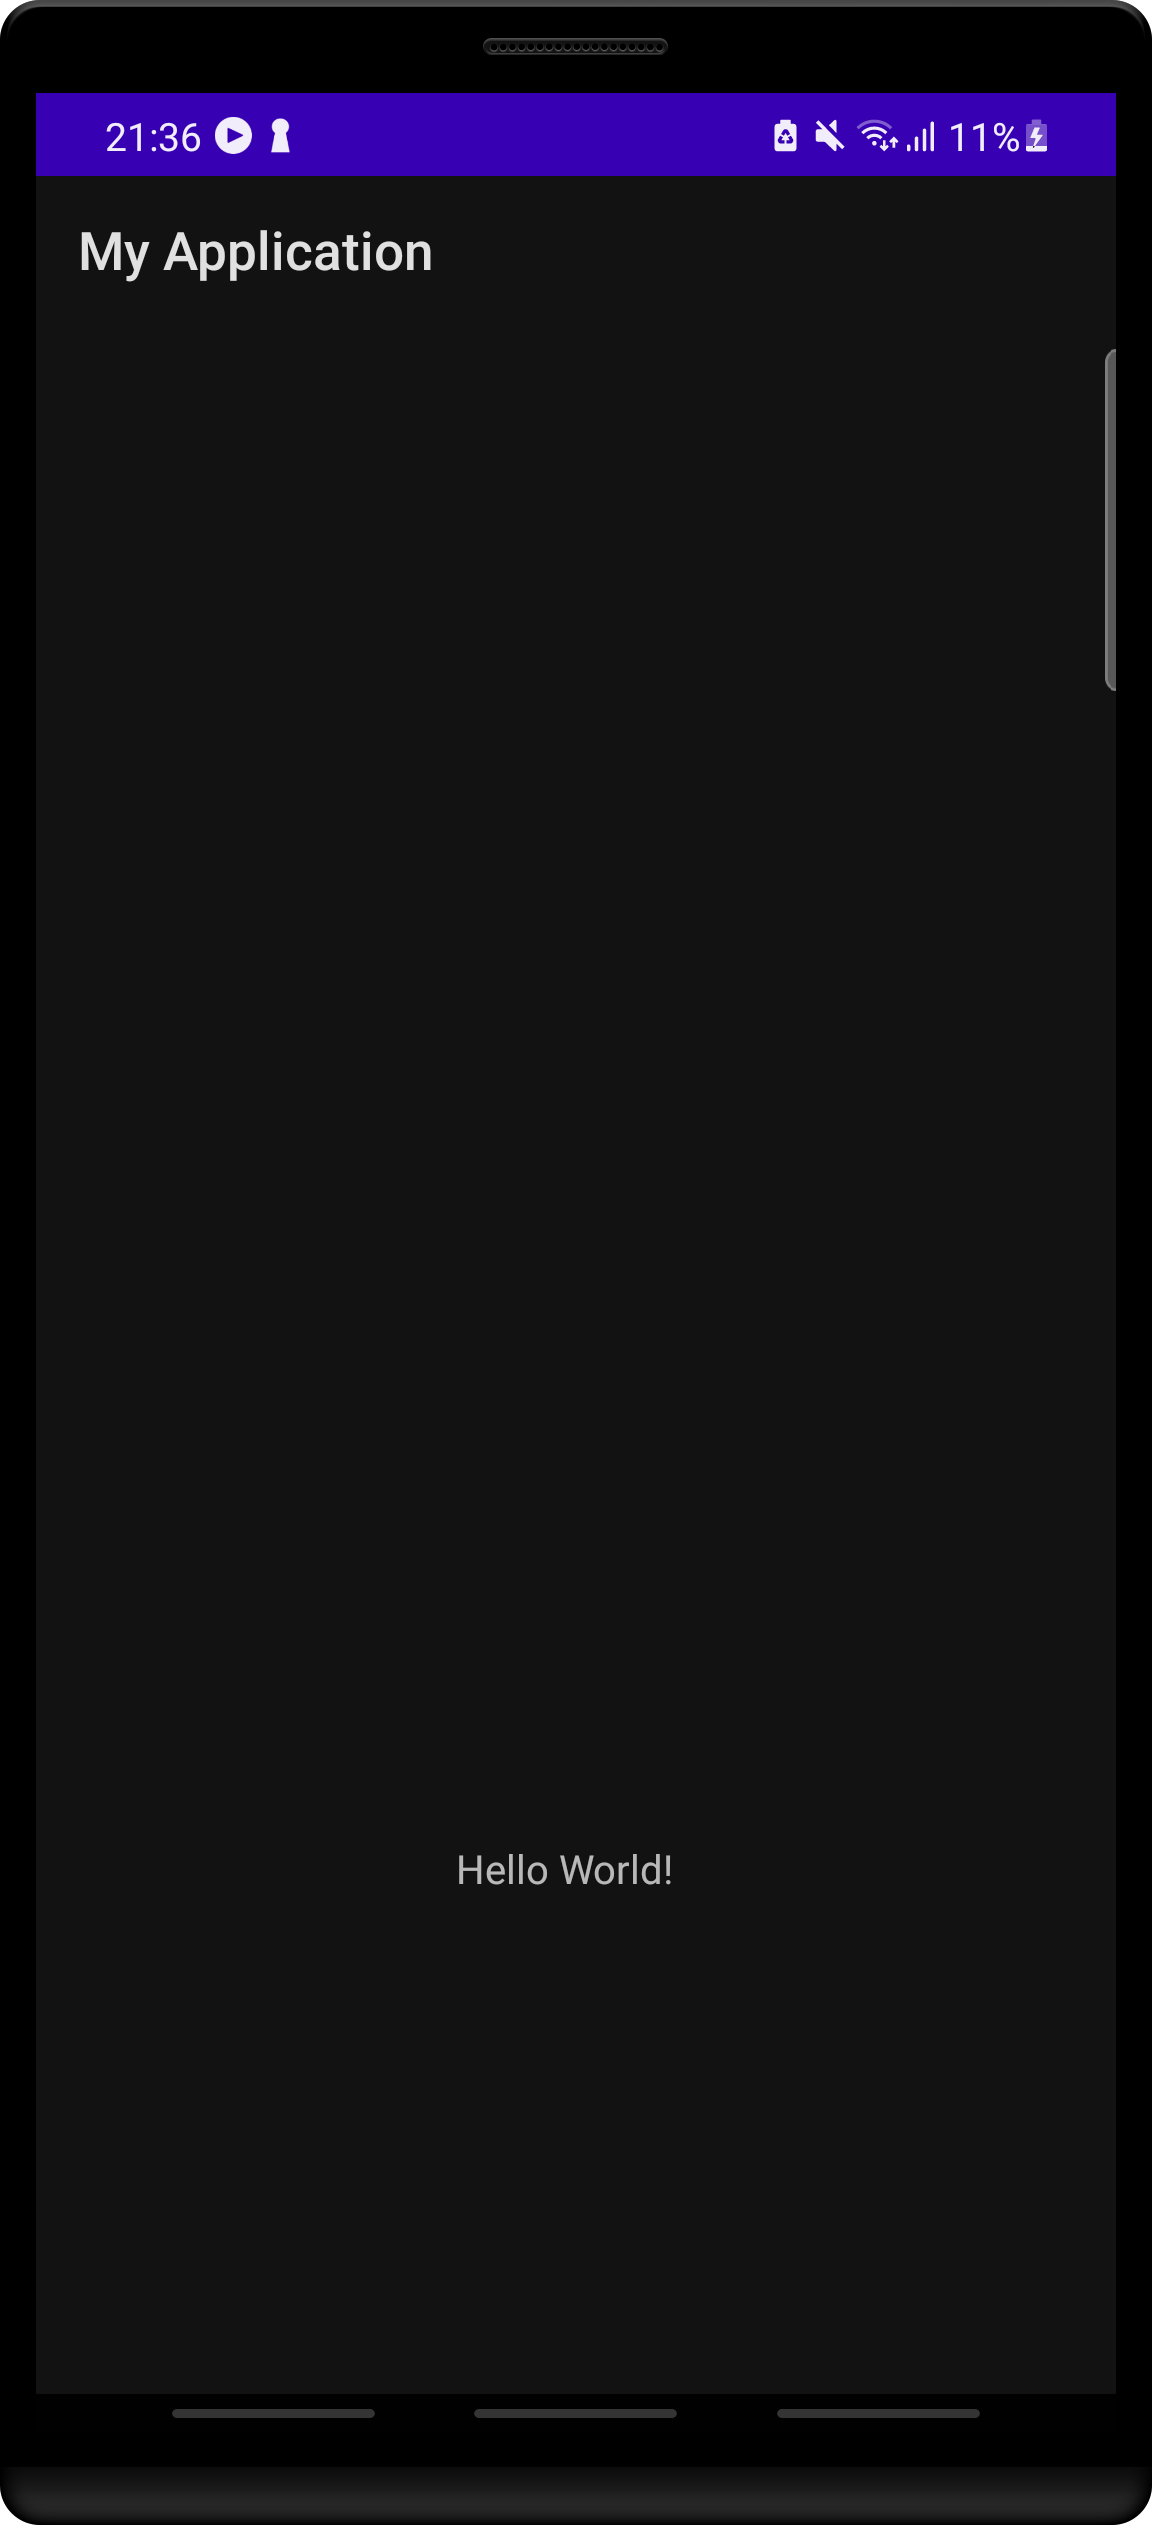
\includegraphics[height=0.9\textwidth]{captureHelloWorldAppPhone}
  \paragraph{}
  Tout d'abord, dans un fichier .xml dans res/layout, nous déclarons une balise \textbf{<TextView>} avec un attribut \textbf{android:text} qui a pour valeur "Hello World!".
  \newline\newline
  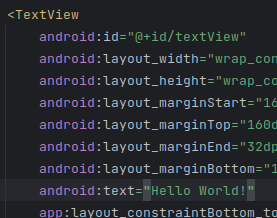
\includegraphics[width=.49\textwidth]{screenshotHelloWorldLayout}
  % 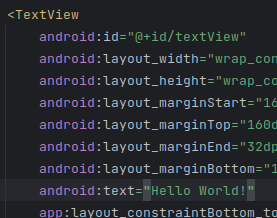
\includegraphics[width=.457\textwidth]{screenshotHelloWorldLayout}
  \newline
  
  Afin de l'afficher à l'écran on va utilser ce \textbf{layout} dans une activité à l'aide de la fonction \textbf{setContentView()}.
  \newline

  Il est également nécessaire d'indiquer à l'application l'activité à lancer comme point d'entrée. Pour cela, dans le manifest, nous ajoutons la balise \textbf{<intent-filter>}, voir figure \ref{fig:manifestHelloWorld} (page \pageref{fig:manifestHelloWorld}) pour plus de détail.
  \newline
  \newline
  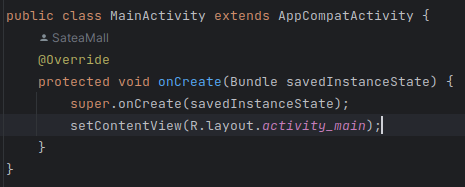
\includegraphics[width=0.49\textwidth]{screenshotCodeHelloWorld.png}
% \end{multicols}
\begin{figure*}
  \centering
  \caption{Manifest pour l'application HelloWorld}
  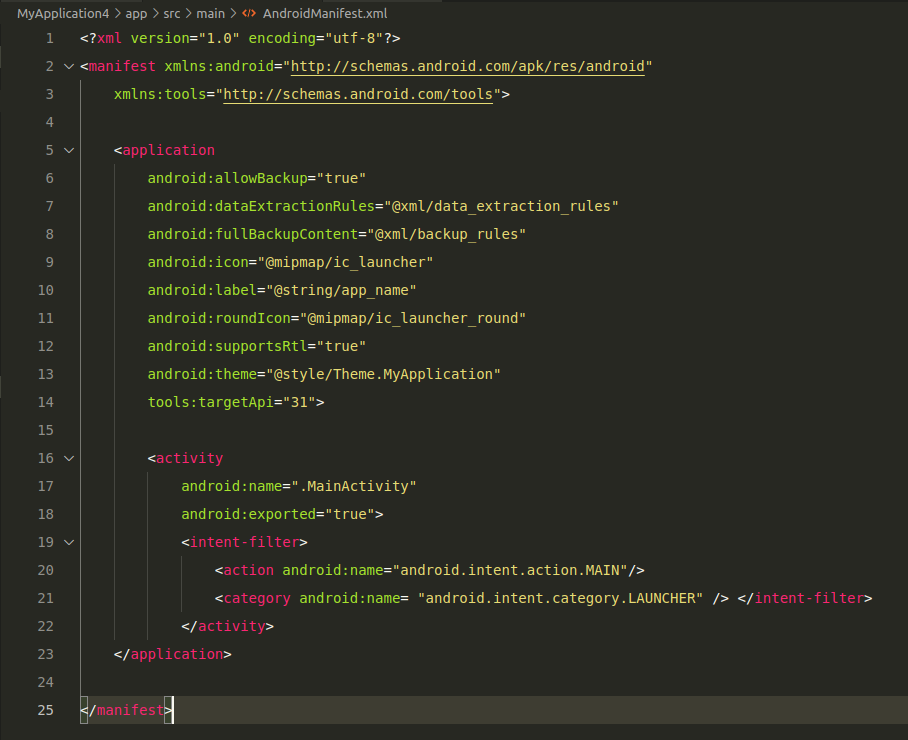
\includegraphics[width=.7\textwidth]{screenshotHelloWorldManifest.png}
  \label{fig:manifestHelloWorld}
\end{figure*}
\section{Simple formulaire}  
  \paragraph{}
  Nous allons voir comment faire une application android réalisant un formulaire où l'on demandera des informations de différentes nature à l'utilisateur.
  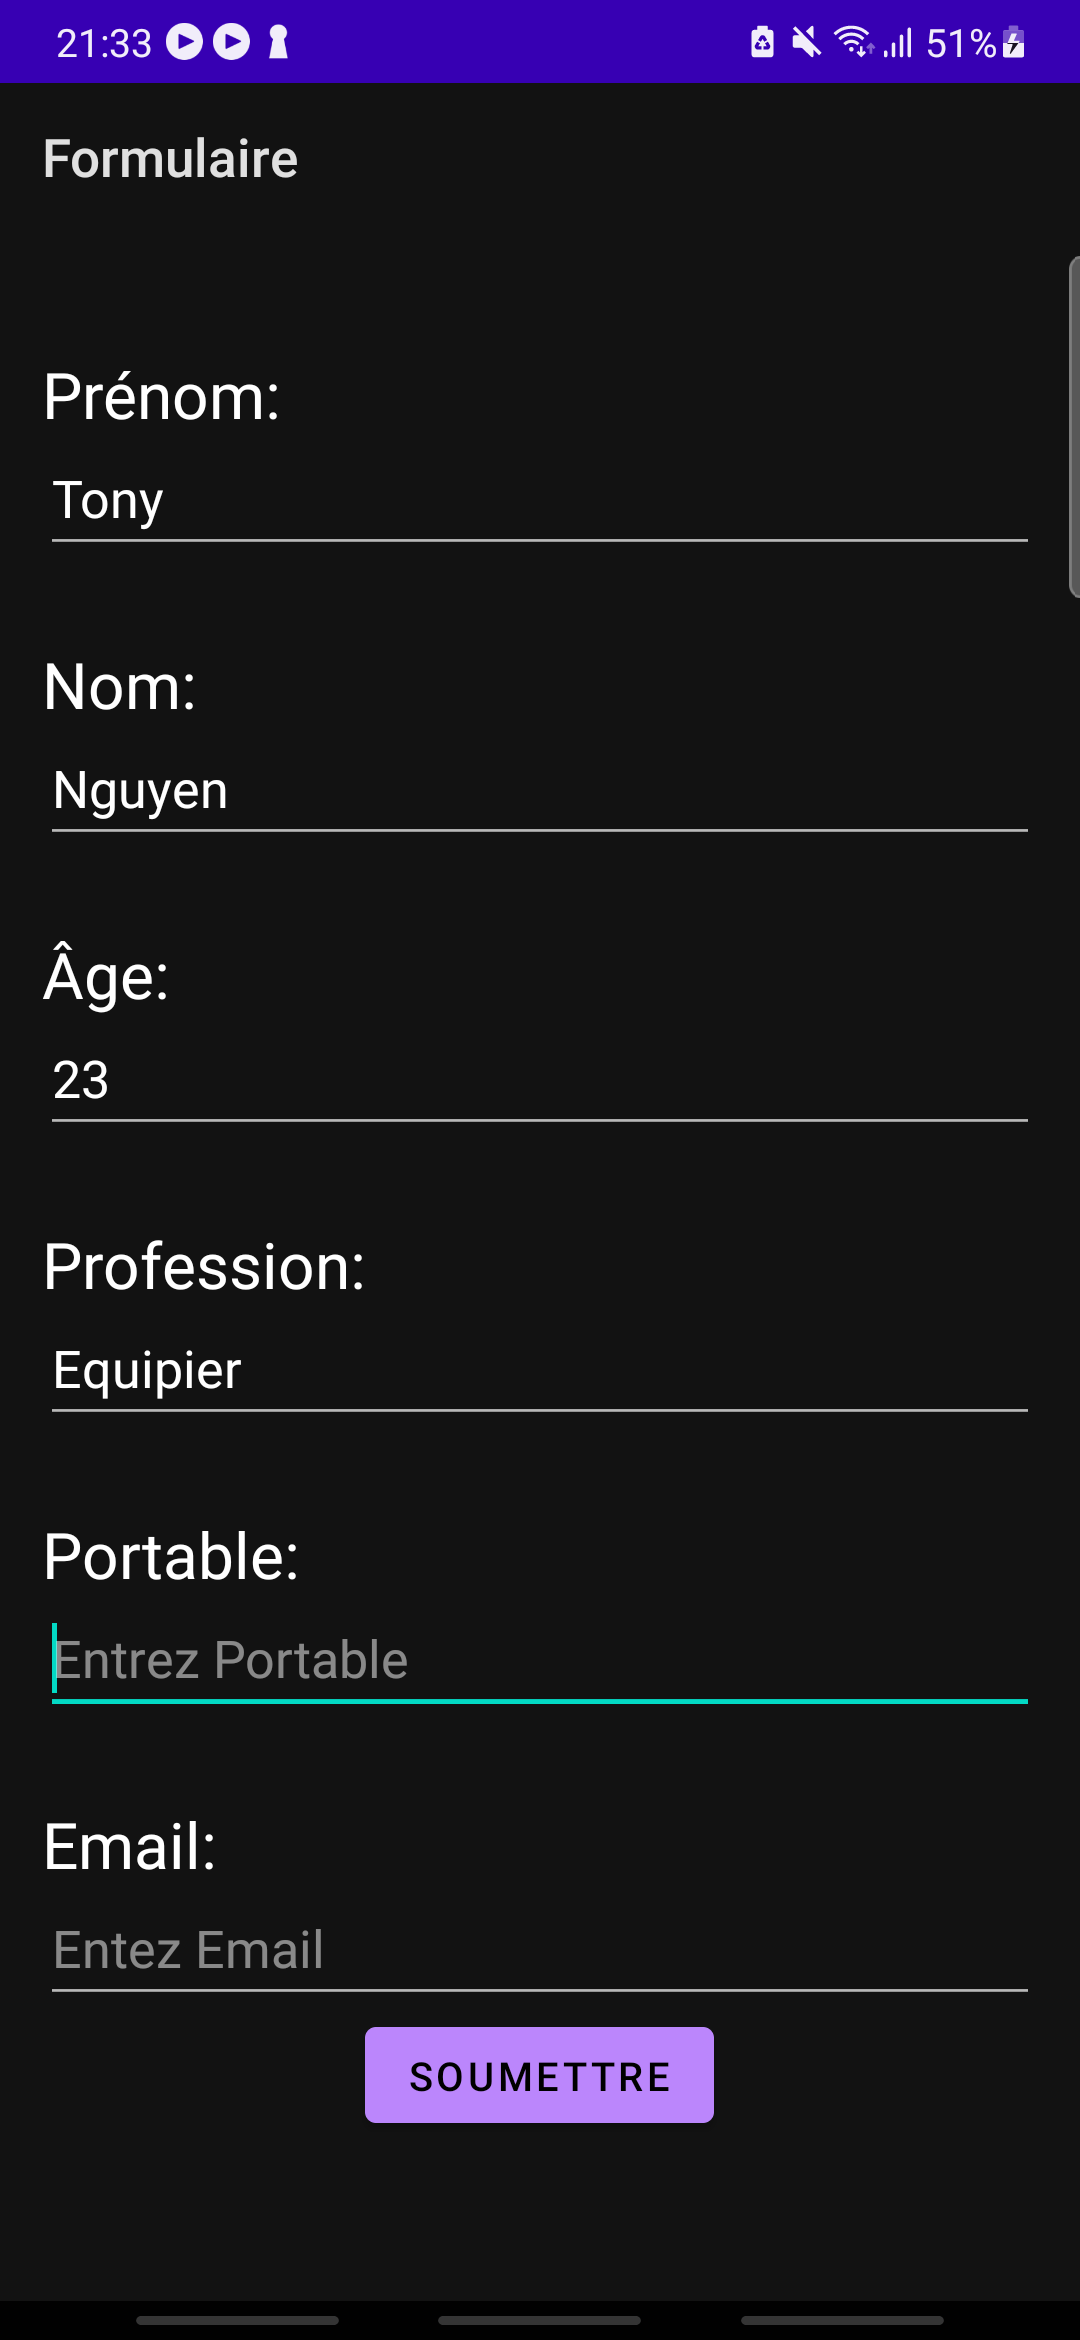
\includegraphics[width=0.49\textwidth]{screenshotFormulaireIncomplet}
  \paragraph{}
  Afin d'implémenter chaque question de notre formulaire, nous utilisons dans notre layout les balises \textbf{<editText>} pour créer un champ de saisie et \textbf{<TextView>} pour l'étiquette associé.
  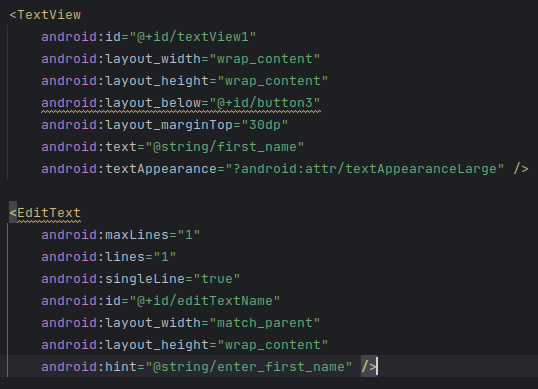
\includegraphics[width=0.49\textwidth]{screenshotFormulaireLayout}

  \subsection{Internationalisation}
  \paragraph{}
    Le système Android étant largement répandu dans le monde, il est préferable de prévoir plusieurs traduction pour des utilisateurs à l'international. Nous allons voir comment.
  \paragraph{}
    Pour cela nous allons utiliser le concept de \textbf{ressources}.  

    Remarquons que dans le fichier de layout, dans les balises, les attributs text et hint n'ont pas de concrète mais plutot \textbf{une référence (@type/name)}. \par
    Dans res/values/strings.xml et res/values/fr/strings.xml, nous déclarons les différents valeurs, mais avec le même attribut name. 
    
    En changeant la langue du système globale, l'application sera choisir entre le fichier strings.xml par défaut ou fr/strings.xml si le sytème est en français.
  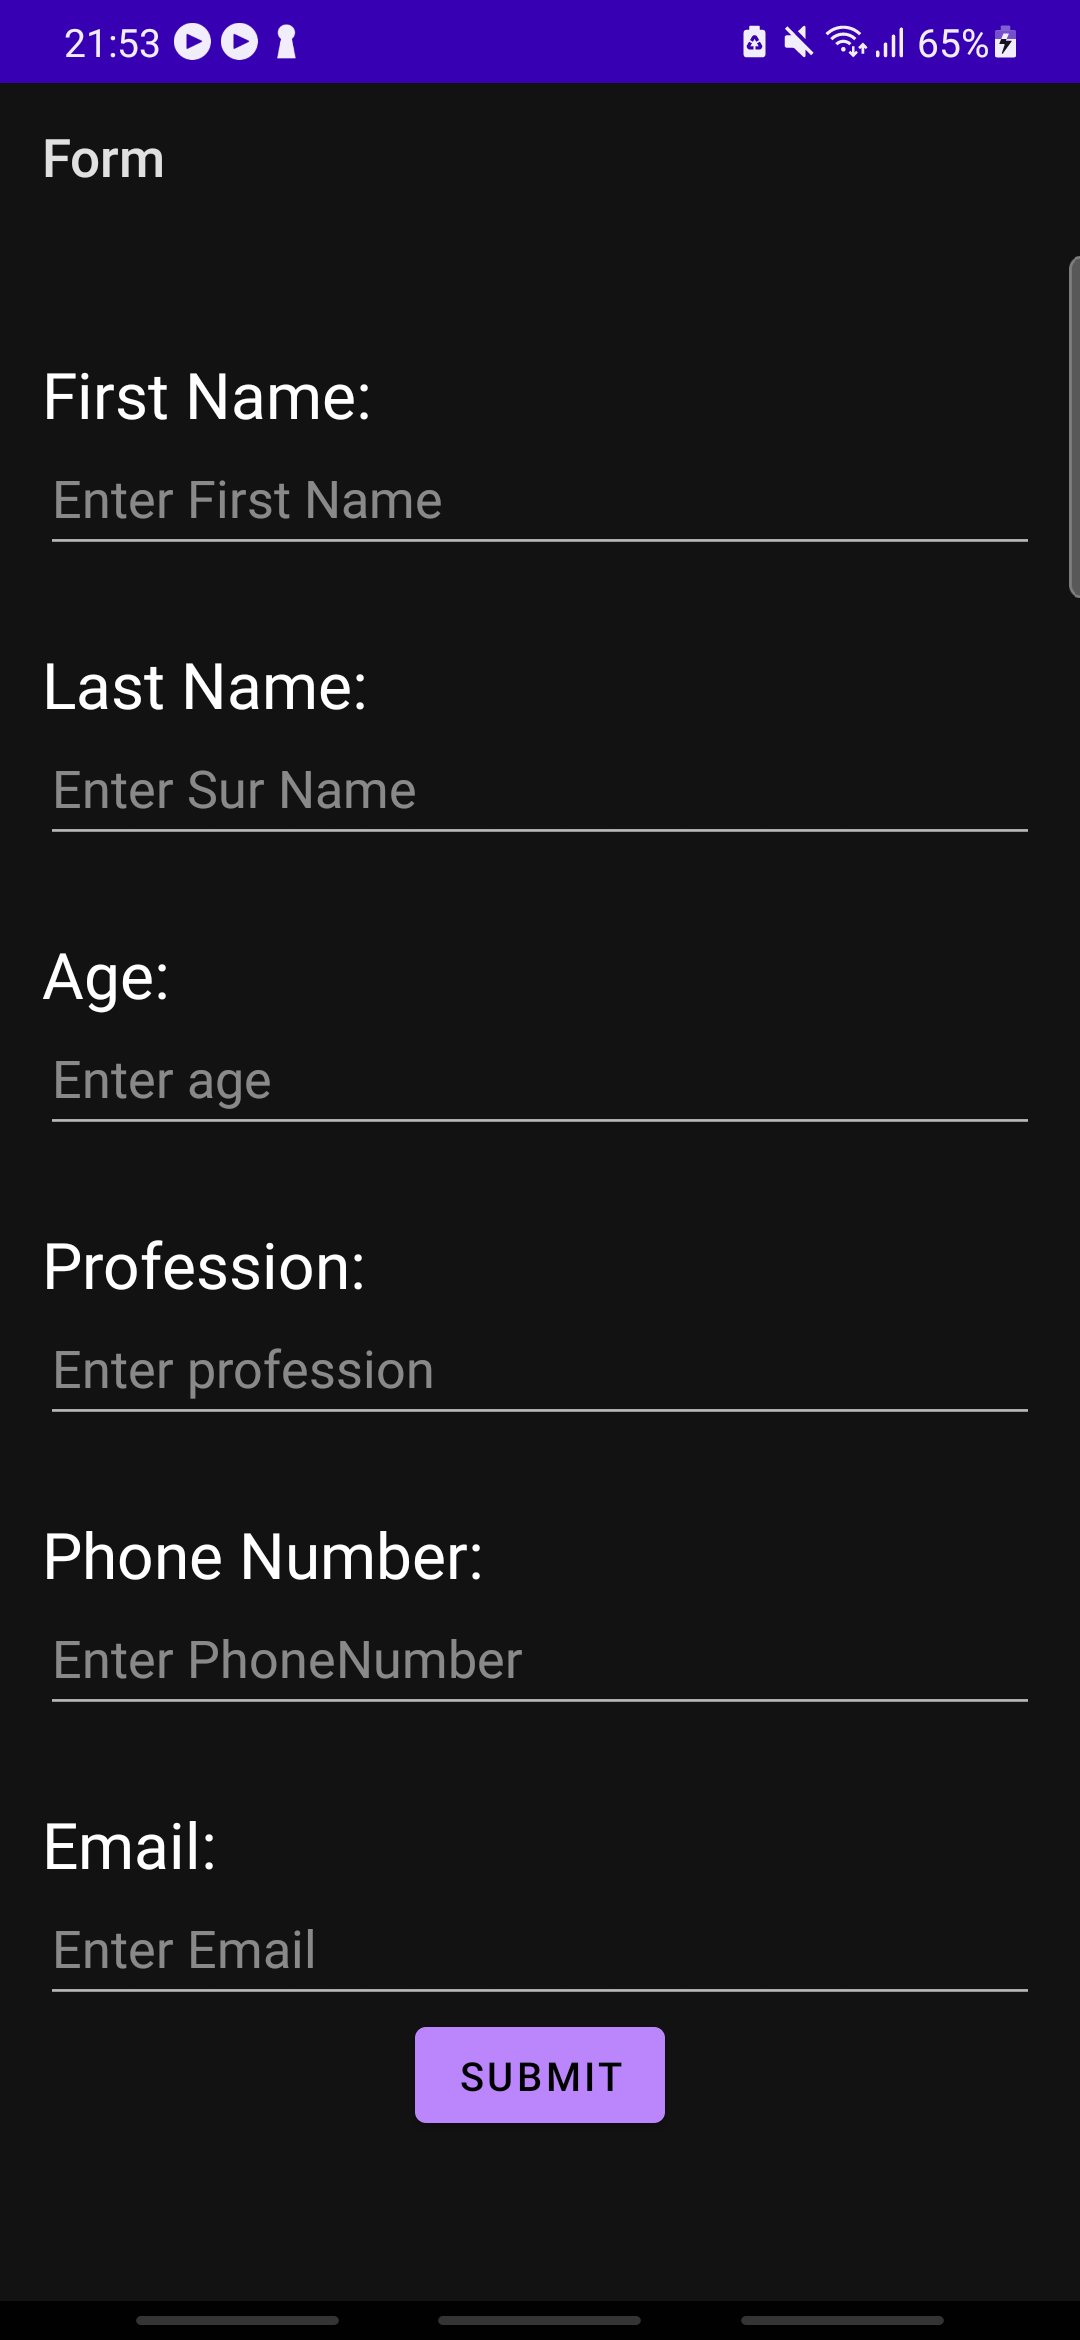
\includegraphics[width=0.49\textwidth]{screenshotFormulaireInternational}
  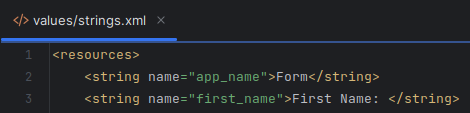
\includegraphics[width=0.49\textwidth]{international/ressourcesEn}
  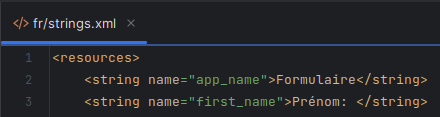
\includegraphics[width=0.49\textwidth]{international/ressourcesFr}
  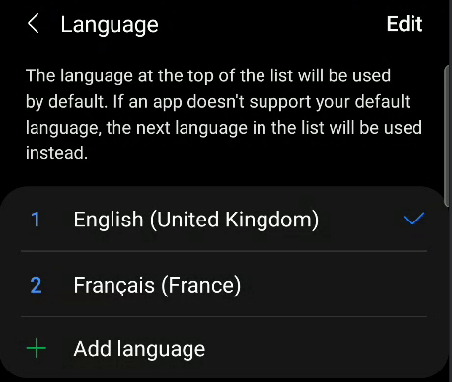
\includegraphics[width=0.49\textwidth]{international/settings}
  
  \subsection{Évenements}
    \paragraph{}
      À présent, nous allons découvrit de quel façon réagir lors de l'action utilisateur "appuyer sur un bouton".
    \paragraph{}
      Avant tout, il est nécessaire de récuper l'objet représentant le boutton. Une fois récupérer, nous allons pouvoir lui ajouter \textbf{un listener} afin qu'il réagisse à un appuie avec la fonction \textbf{setOnClickListener}. Nous lui donnons en argument une sous classe de OnClickListener en créant une classe anonyme héritant de OnClickListener dans laquelle nous \textbf{redéfinissons onClick()}. C'est dans cette fonction que nous pouvons décider quelles actions prendre lors de cet évènements.

      Nous choissisons comme comportement du boutton, une simple demande de confirmation ou d'annulation. Cela est présenter sous la forme d'une fenêtre de dialogue. Android nous permet d'en créer une comme ceci : "new AlertDialog.Builder().show();"
      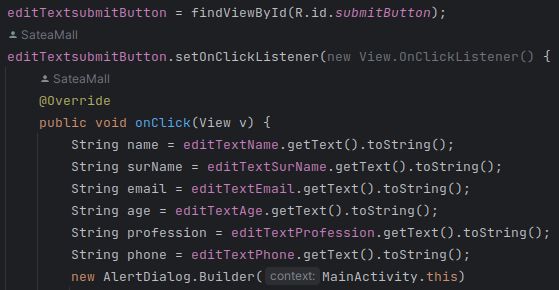
\includegraphics[width=0.49\textwidth]{event/code}
      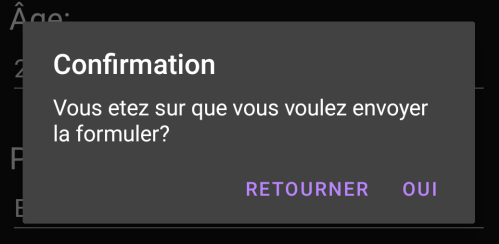
\includegraphics[width=0.49\textwidth]{event/dialogue}
  
  \subsection{Intent explicite}
    \paragraph{}
      Qu'est ce qu'un "Intent" ? 

      Un Intent est un objet représentant la communication entre composant sur Android. Il représente une demande d'opération à exécuter. Il permet notamment de démarer des d'autres composants/application.

      Dans un Intent \textbf{explicite}, l'activité à démarer est \textbf{explicitement nommé}. 

      Tout d'abord voyons ensemble les intents explicite.
    \paragraph{}
      En effet, comme nous pouvons le remarqué, dans le constructeur le l'Intent, nous mettons en second paramètre la classe de l'activité à démarer. La méthode \textbf{putExtra} nous permet va nous permettre de transmettre des informations à l'activité à démarrer. Pour effectivement lancer cette nouvelle activité, il nous suffit de faire \textbf{startActivity(uneIntent)}.
      \includegraphics[width=0.49\textwidth]{explicit/implementation}
      % 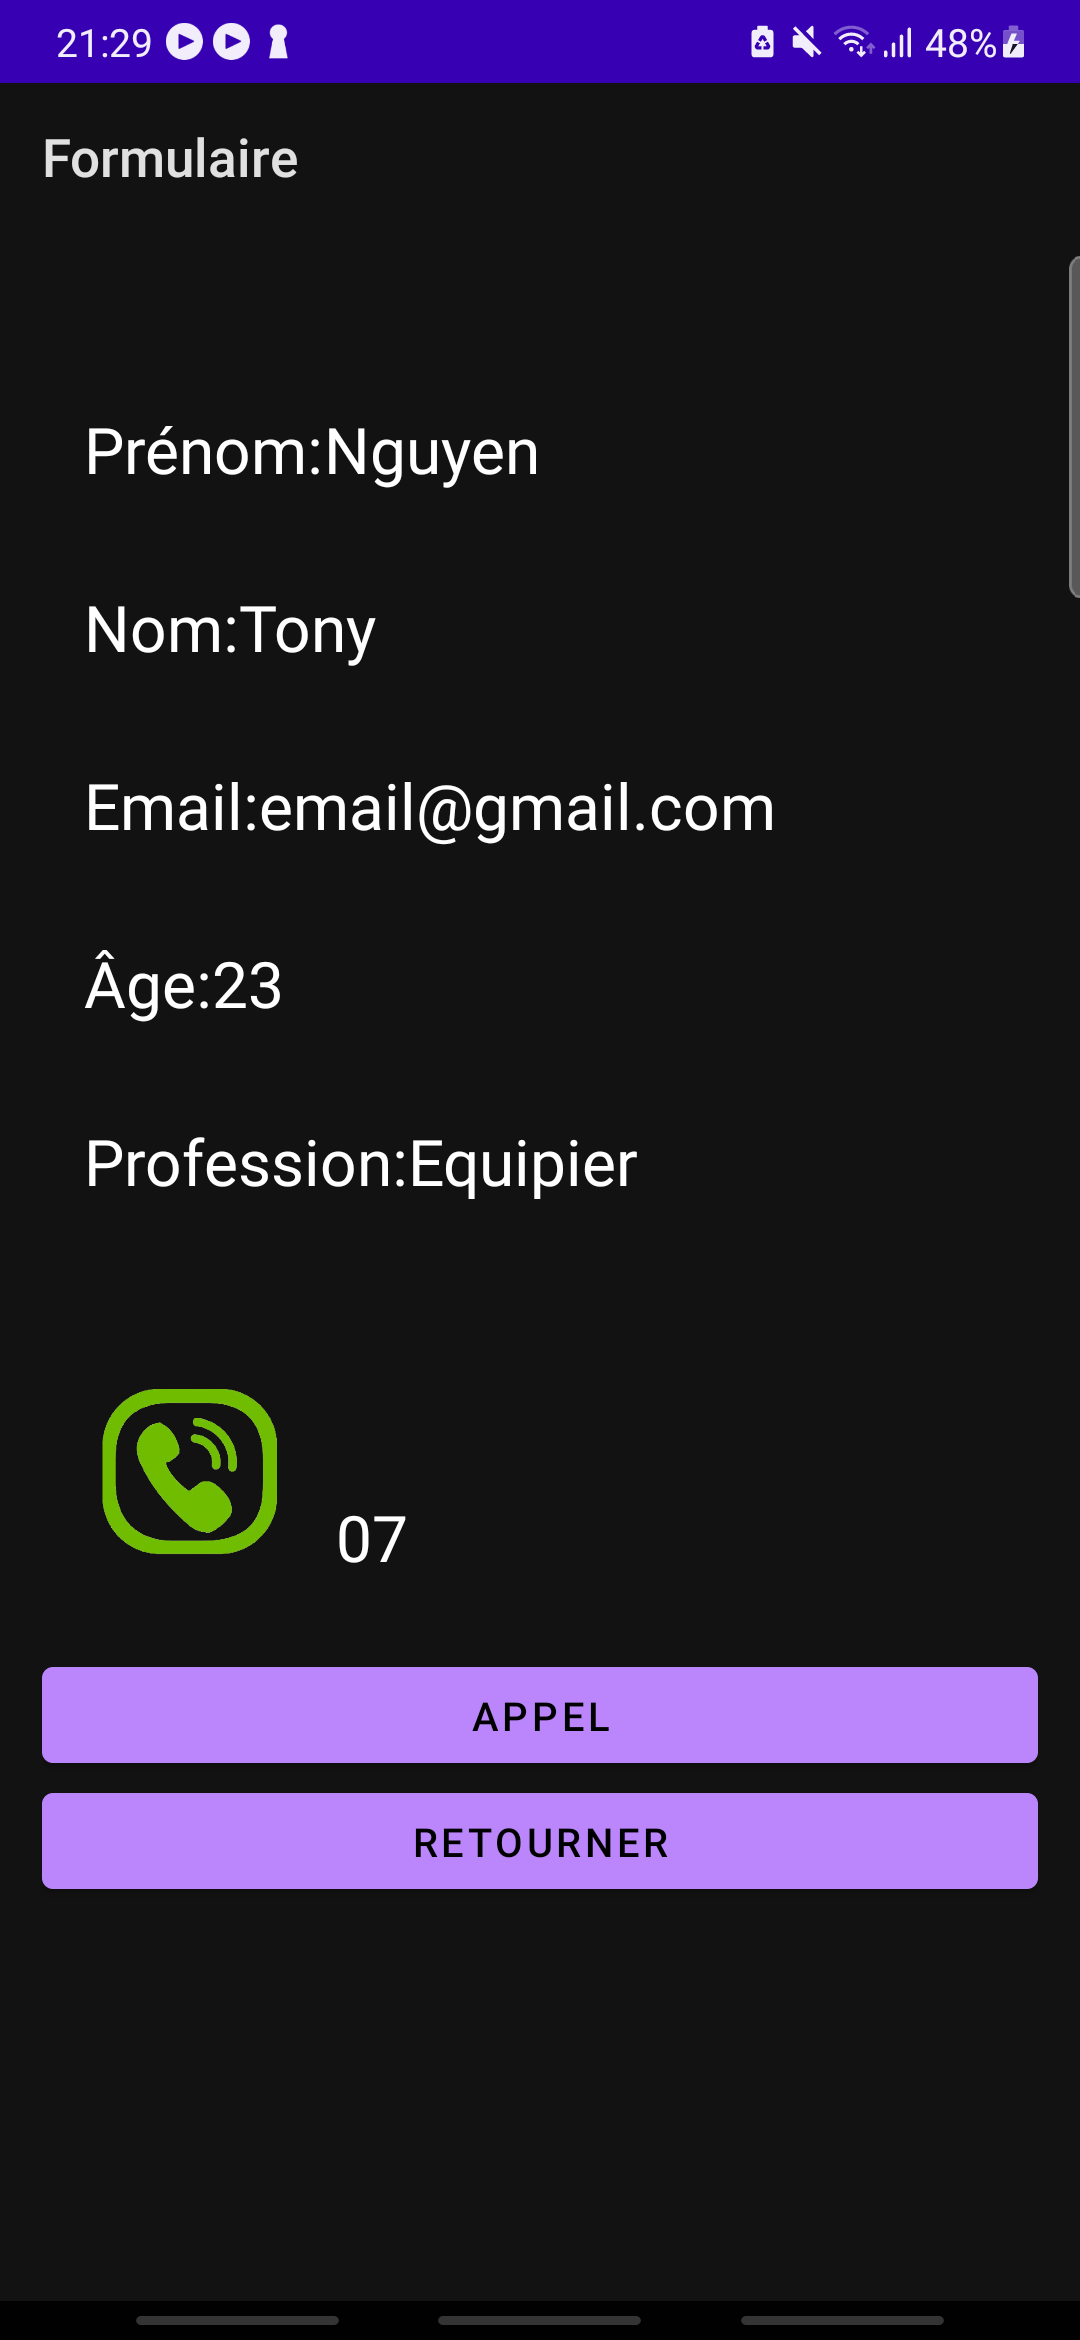
\includegraphics[width=0.49\textwidth]{explicit/screenshotFormulaireAffichage}
    \subsection{Intent implicite}
      \paragraph{}
        Nous allons maintenant voir les intents implcite qui eux \textbf{ne nécessite pas de nommer l'activité à démarer}.
      \paragraph{}
        Comme on peut le voir sur l'image ci-dessous, nous n'indiquons pas le nom de l'activité à démarrer, seulement l'action à réaliser.
      \includegraphics[width=0.49\textwidth]{implicit/implementation}
      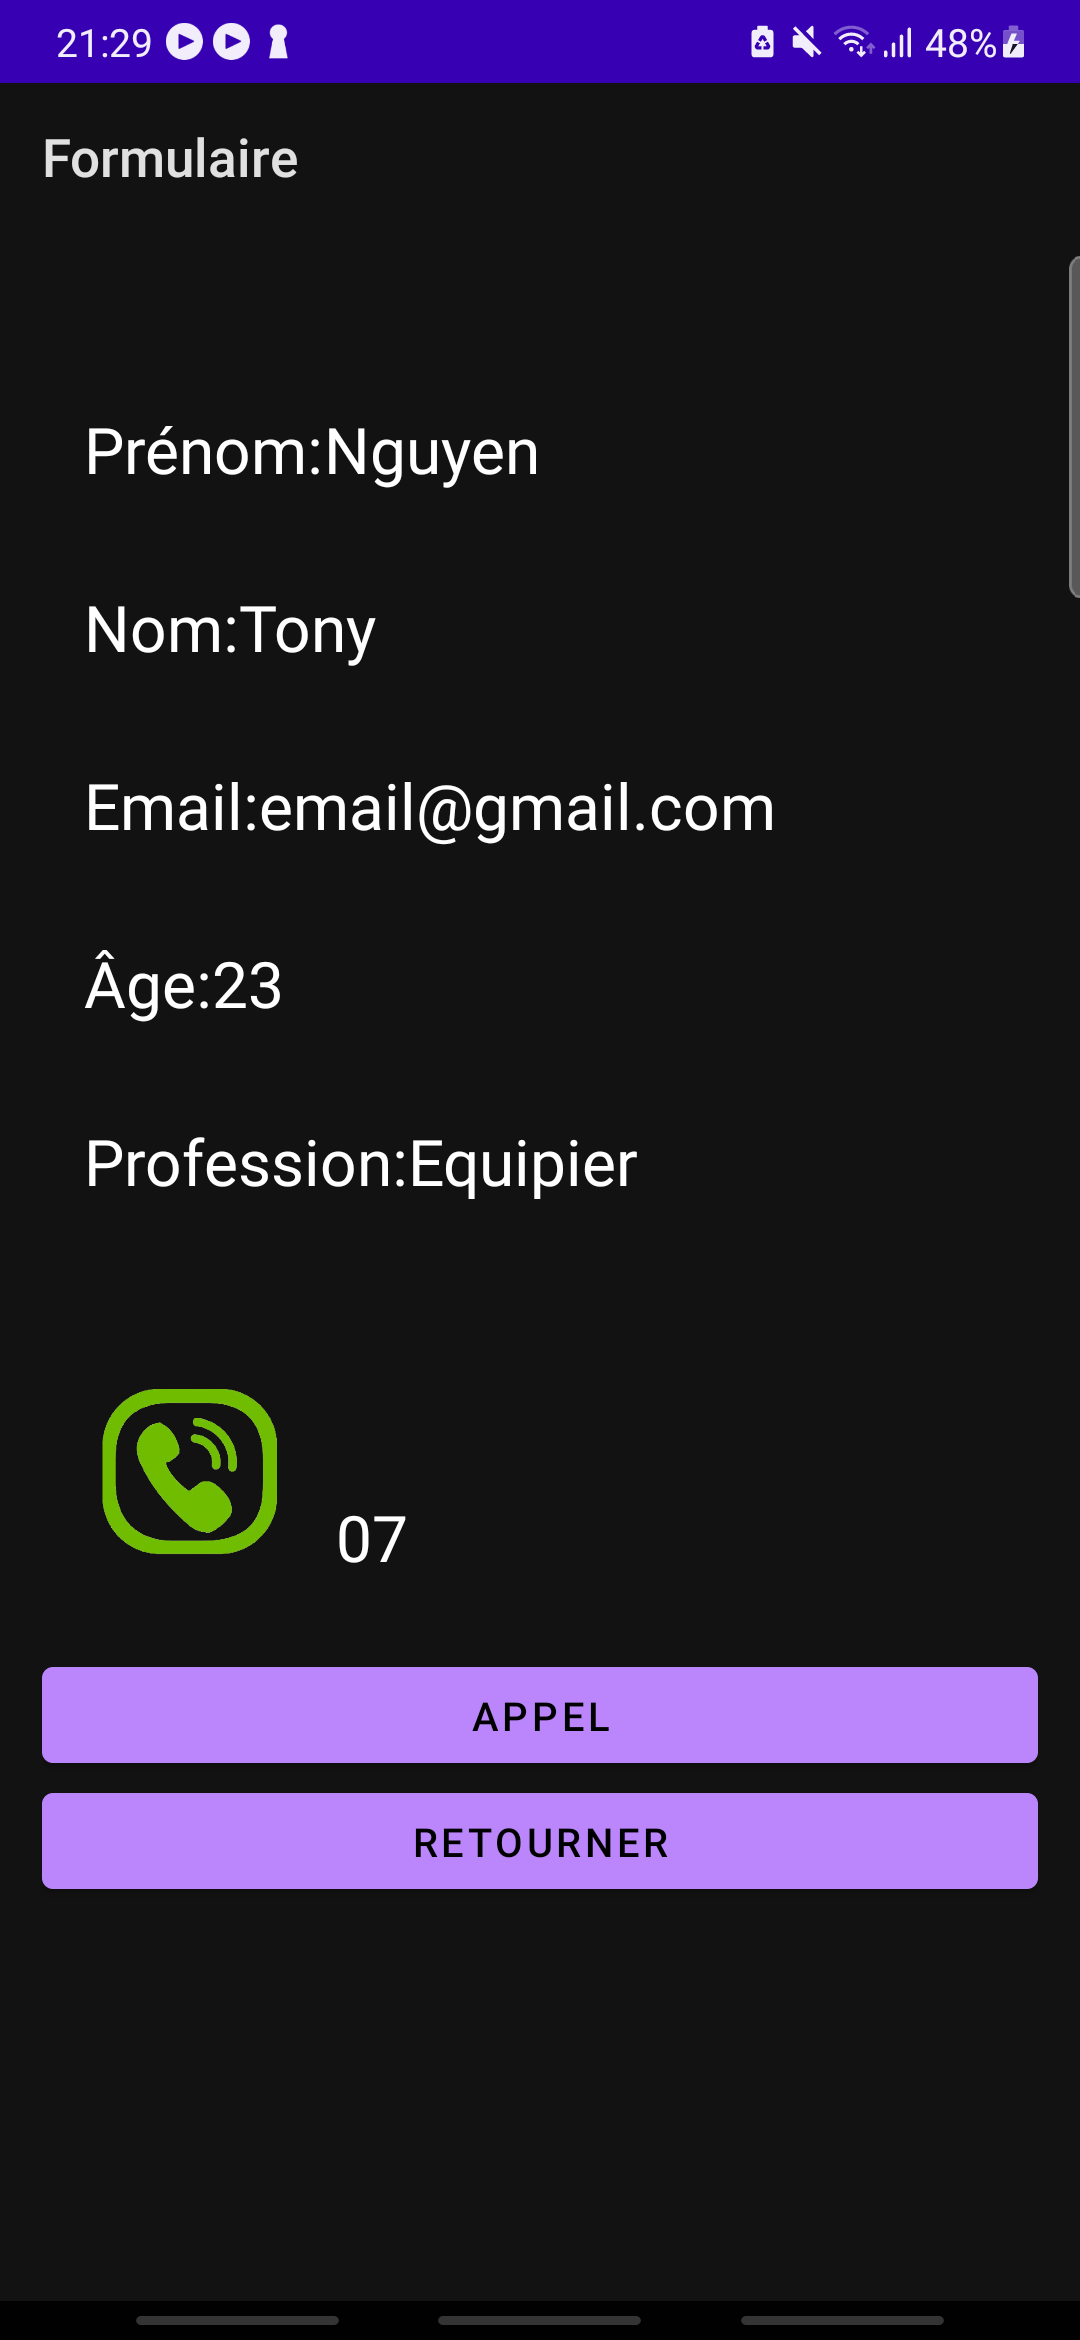
\includegraphics[width=0.49\textwidth]{explicit/screenshotFormulaireAffichage}
      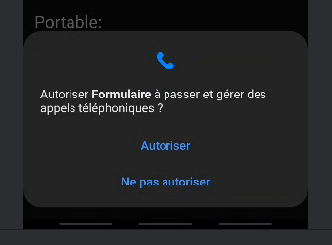
\includegraphics[width=0.49\textwidth]{implicit/appel}
  \section{Consultation les horaires de trains}
    \paragraph{}
      Nous allons faire une application pour consulter des horaires de trains.
    \begin{figure*}
      \centering
      \caption{Diagramme de classe de l'application Trains}
      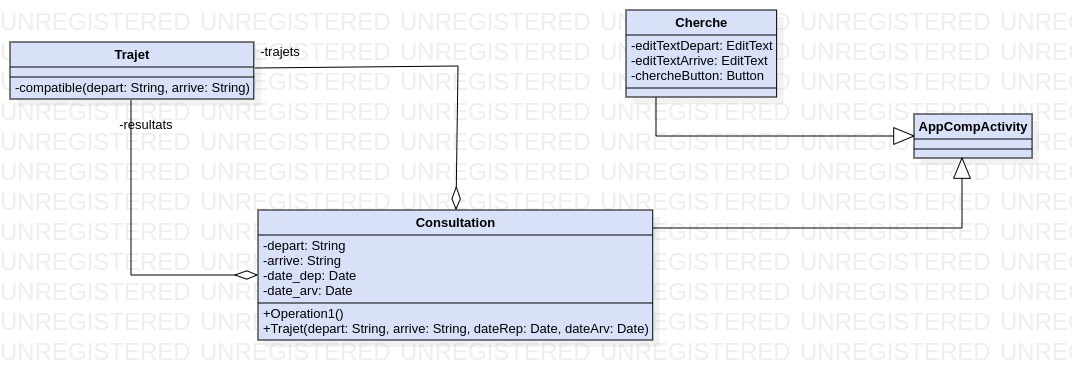
\includegraphics[width=\textwidth]{jpg/Model1!Train_1}
      \label{fig:manifestHelloWorld}
    \end{figure*}
  \section{Simple d’agenda}
    \paragraph{}
      Nous allons réalisé une application d'agenda.
    \begin{figure*}
      \centering
      \caption{Diagramme de classe de l'application Agenda}
      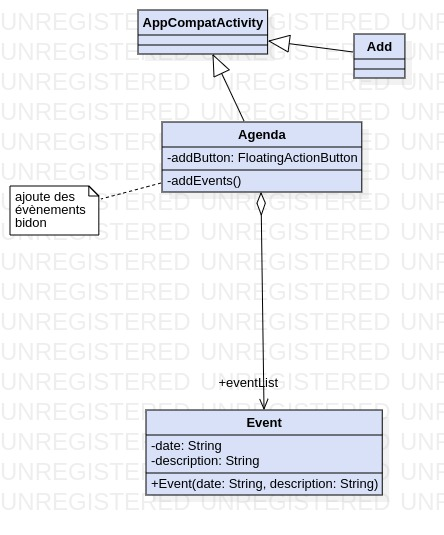
\includegraphics[width=\textwidth]{jpg/Model!Agenda_0}
      \label{fig:manifestHelloWorld}
    \end{figure*}
  \end{multicols}
\end{document}